% !TeX spellcheck = es_ES
% Chapter 1

%\chapter{Chapter Title Here} % Main chapter title
%
%\label{Chapter1} % For referencing the chapter elsewhere, use \ref{Chapter1} 

%----------------------------------------------------------------------------------------

% Define some commands to keep the formatting separated from the content 
\newcommand{\grad}[0]{$^\circ$C}
%\newcommand{\tabhead}[1]{\textbf{#1}}
%\newcommand{\code}[1]{\texttt{#1}}
%\newcommand{\file}[1]{\texttt{\bfseries#1}}
%\newcommand{\option}[1]{\texttt{\itshape#1}}

%----------------------------------------------------------------------------------------

\chapter{Control de la temperatura}
	El sistema cuenta con dos calentadores de precisión al interior del baño termostatado de 25 litros. Estos calentadores junto con el ba\~no externo determinan la temperatura de trabajo del equipo. El ba\~no externo se usa con el objetivo de mantener siempre activos los calentadores internos en alg\'un nivel de potencia intermedio, pues el ba\~no externo, al tener una temperatura inferior agregar una carga permanente a los calentadores internos \cite{Suurkuusk}. Para monitorear la temperatura del ba\~no el calor\'imetro cuenta con dos termistores, el primero para trabajar a temperaturas inferiores a 50 \grad{} y el segundo para temperaturas superiores a este valor. La se\~nal generada por uno de estos termistores se compara con un valor de resistencia definido por el usuario. La resistencia y por ende la temperatura del equipo se fijan usando cuatro resistencias de década, esto es que cada resistencia es una potencia de 10 menor que la anterior, las cuales se encuentran en la parte inferior del calor\'imetro, en la \autoref{fig: decadeResistors} corresponden A, B, C, y D, de esta manera se pueden realizar experimentos a temperaturas en el rango de 5 a 80 \grad{}. El diagrama del sistema de control t\'ermico del calor\'imetro se muestra en el \autoref{anx: imagenes} como \autoref{fig: controlTermico}.
	
	\begin{figure}[h]
		\centering
		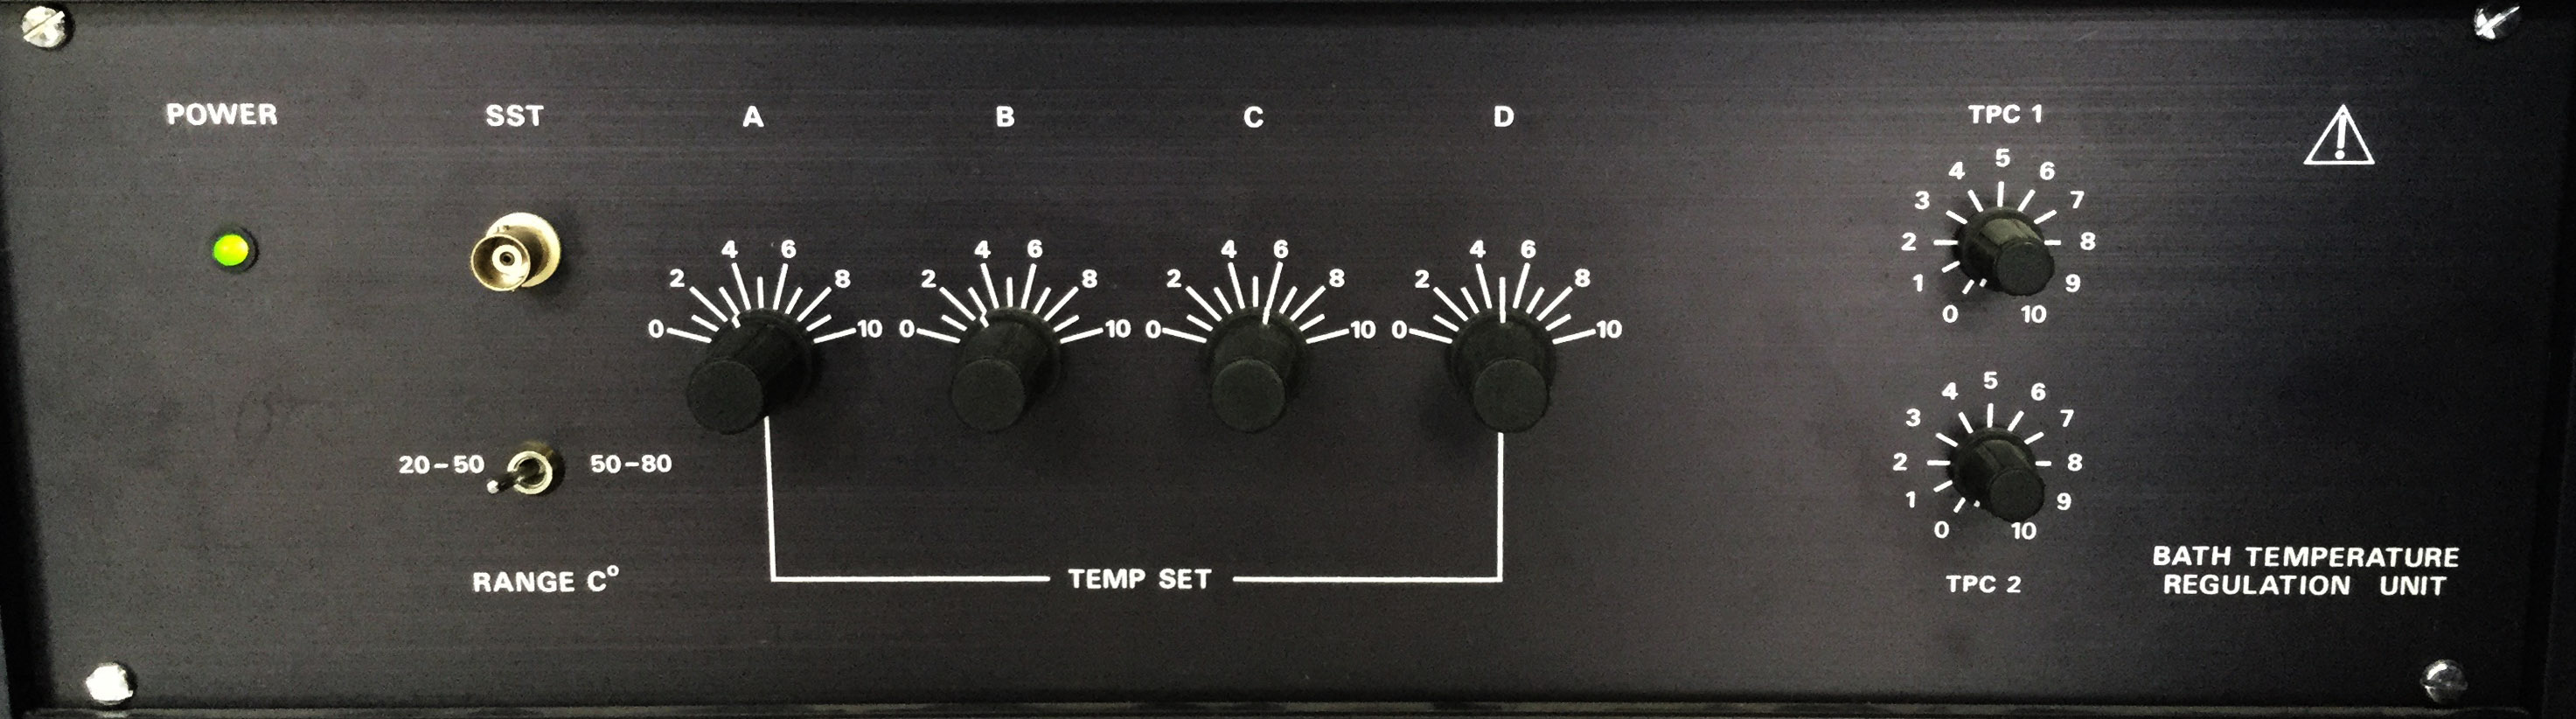
\includegraphics[width=0.7\linewidth]{Figures/decadeResistors}
		\caption{Resistencias de década que controlan la temperatura.}
		\label{fig: decadeResistors}
	\end{figure}
	
	Para determinar la equivalencia de resistencia y temperatura el calorímetro cuenta con una tabla que relaciona los valores de resistencia y temperatura de ba\~no externo que dan lugar a una temperatura constante en el ba\~no interno. Dicha tabla se muestra en el \autoref{ch: imagenes} como \autoref{fig: temperatureTable}, sin embargo, el uso de esa tabla est\'a limitado a temperaturas ambiente superiores a 20 \grad{} por lo cual, en el caso particular de Bogot\'a rara vez se cumplen. Lo anterior es relevante dado que la resistencia el\'ectrica depende de la temperatura, en el caso de materiales met\'alicos, la resistencia aumenta con la temperatura, y para semiconductores se tiene el efecto contrario \cite{simon2013oxford}.
	
	Una vez realizadas las conexiones el\'ectricas del calor\'imetro para su funcionamiento a 110 VAC, y antes de realizar una calibraci\'on qu\'imica fue necesario estabilizar el equipo a una temperatura de 25 \grad{}, puesto que el objetivo de la calibraci\'on qu\'imica es contrastar los datos obtenidos con el calor\'imetro con los reportados en la literatura, los cuales por convenci\'on se reportan a estas condiciones. Para alcanzar esta temperatura se probó con las condiciones reportadas en la \autoref{fig: temperatureTable}, en donde los valores de cada resistencia de década se muestra a continuación. 
	\begin{table}[h]
		\centering
		\caption{Valores de las resistencias de década, para una temperatura de 25 \grad{}, seg\'un calibración original del calorímetro.}
		\begin{tabular}{r|cccc|l}
			\hline
			\textbf{Baño interno (\grad{})} & A ($10^4$ $\Omega$) & B ($10^3$ $\Omega$) & C ($10^2$ $\Omega$) & D ($10^1$ $\Omega$) & \textbf{Baño externo (\grad{})} \\
			\hline
			25.0 & 3 & 2 & 4 & 9 & 22.0 \\
			\hline
		\end{tabular}
		\label{tb: decadeResistorsBefore}
	\end{table}
	
	La temperatura del equipo fue monitoreada por cuatro días, con al menos un registro diario, los resultados se muestran en la \autoref{tb: temperatureRegister}. En ella se puede observar que cuando inicialmente se creía que la temperatura del baño estaba cerca de estabilizarse a 25 \grad{}, en realidad estaba en aumento de la temperatura, y cuando se creía que finalmente el calorímetro se había estabilizado en 26,86 \grad{} el sistema se encontraba oscilando como lo muestra la última temperatura registrada.
	
	\begin{table}[h]
		\centering
		\caption{Registro de temperaturas del baño interno en el tiempo para la configuración recomendada por la calibración en la \autoref{fig: temperatureTable}.}
		\begin{tabular}{r|c}
			\hline
			\textbf{Fecha (DD/MM HH:MM)} & \textbf{Temperatura (\grad{})} \\
			\hline
			07/09 11:13 & 25,14 \\
			07/09 11:50 & 25,19 \\
			10/09 09:43 & 26,64 \\
			11/09 09:22 & 26,86 \\
			11/09 10:00 & 26,86 \\
			12/09 08:30 & 26,86 \\
			12/09 10:30 & 26,86 \\
			12/09 15:48 & 26,64 \\
			\hline
		\end{tabular}
		\label{tb: temperatureRegister}
	\end{table}
	
	Sin embargo, esta no fue la única configuración probada, pues también se trató de estabilizar el equipo usando: 2977 (A,B,C,D), que dio lugar a las siguientes temperaturas de baño interno 25,44 \grad{}, y 28,38 \grad{} luego de 5 días. De manera similar se probaron 3000, 3021, 3040, 3100, 3121, 3140, 3160 ninguna de las cuales presentó una temperatura estable. Debido a la dificultad de estabilizar el equipo a una temperatura determinada, se decidió construir un sistema de monitoreo automatizado para facilitar esta tarea, de esta manera se podría saber el histórico de una configuración, si el sistema está en calentamiento, estable, u oscilando.
	
	\section{Sistema de monitoreo}
	De todas las acciones que se hicieron a lo largo del proyecto, la estabilizaci\'on de la temperatura es la que llev\'o m\'as tiempo. Esto se debi\'o a que existen dos variables que determinan una temperatura en el calor\'imetro, por un lado la configuraci\'on de las resistencias de d\'ecada, y el ba\~no externo, adem\'as se debe tener en cuenta el tiempo de estabilizaci\'on del calor\'imetro, el cual puede tomar cerca de 6 horas en completarse. Para monitorear el estado de la temperatura del ba\~no interno se construy\'o un circuito con tres sensores de temperatura, los sensores LM39 fueron elegidos debido a que presentan una respuesta lineal en voltaje, y tienen un rango de trabajo de 2 \grad{} a 120 \grad{} \cite{instruments1999lm35}. Cada uno de estos sensores fue conectado a tres cables como se muestra en la \autoref{fig: sensors}, y posteriormente fue cubierto con silicona y un cable termoencogible para aislar el sensor del agua. 	
	\begin{figure}[h]
		\centering
		\begin{subfigure}{0.75\textwidth}
			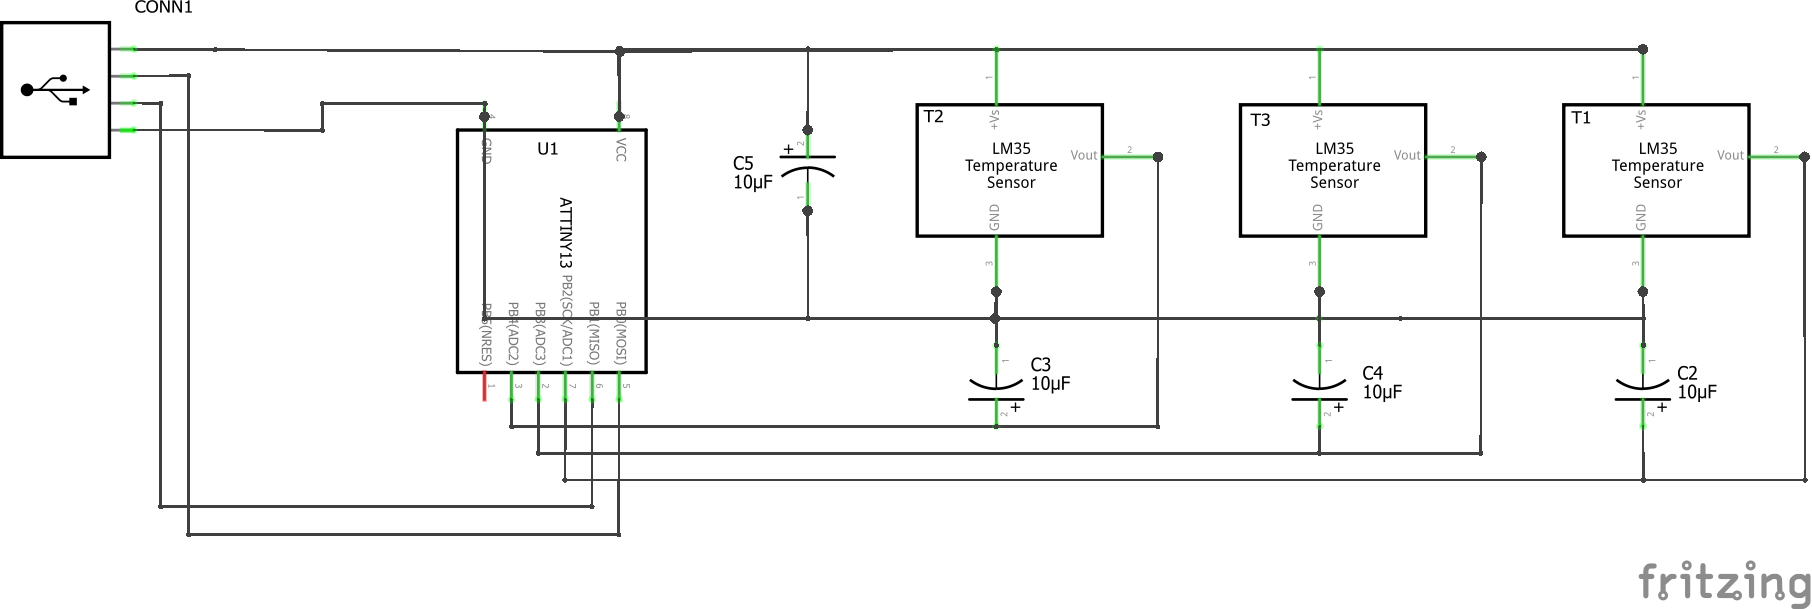
\includegraphics[width=\linewidth]{Figures/Sketch_schem}
			\caption{Conexi\'on al microcontrolador.}	
		\end{subfigure}
		\begin{subfigure}{0.23\textwidth}
			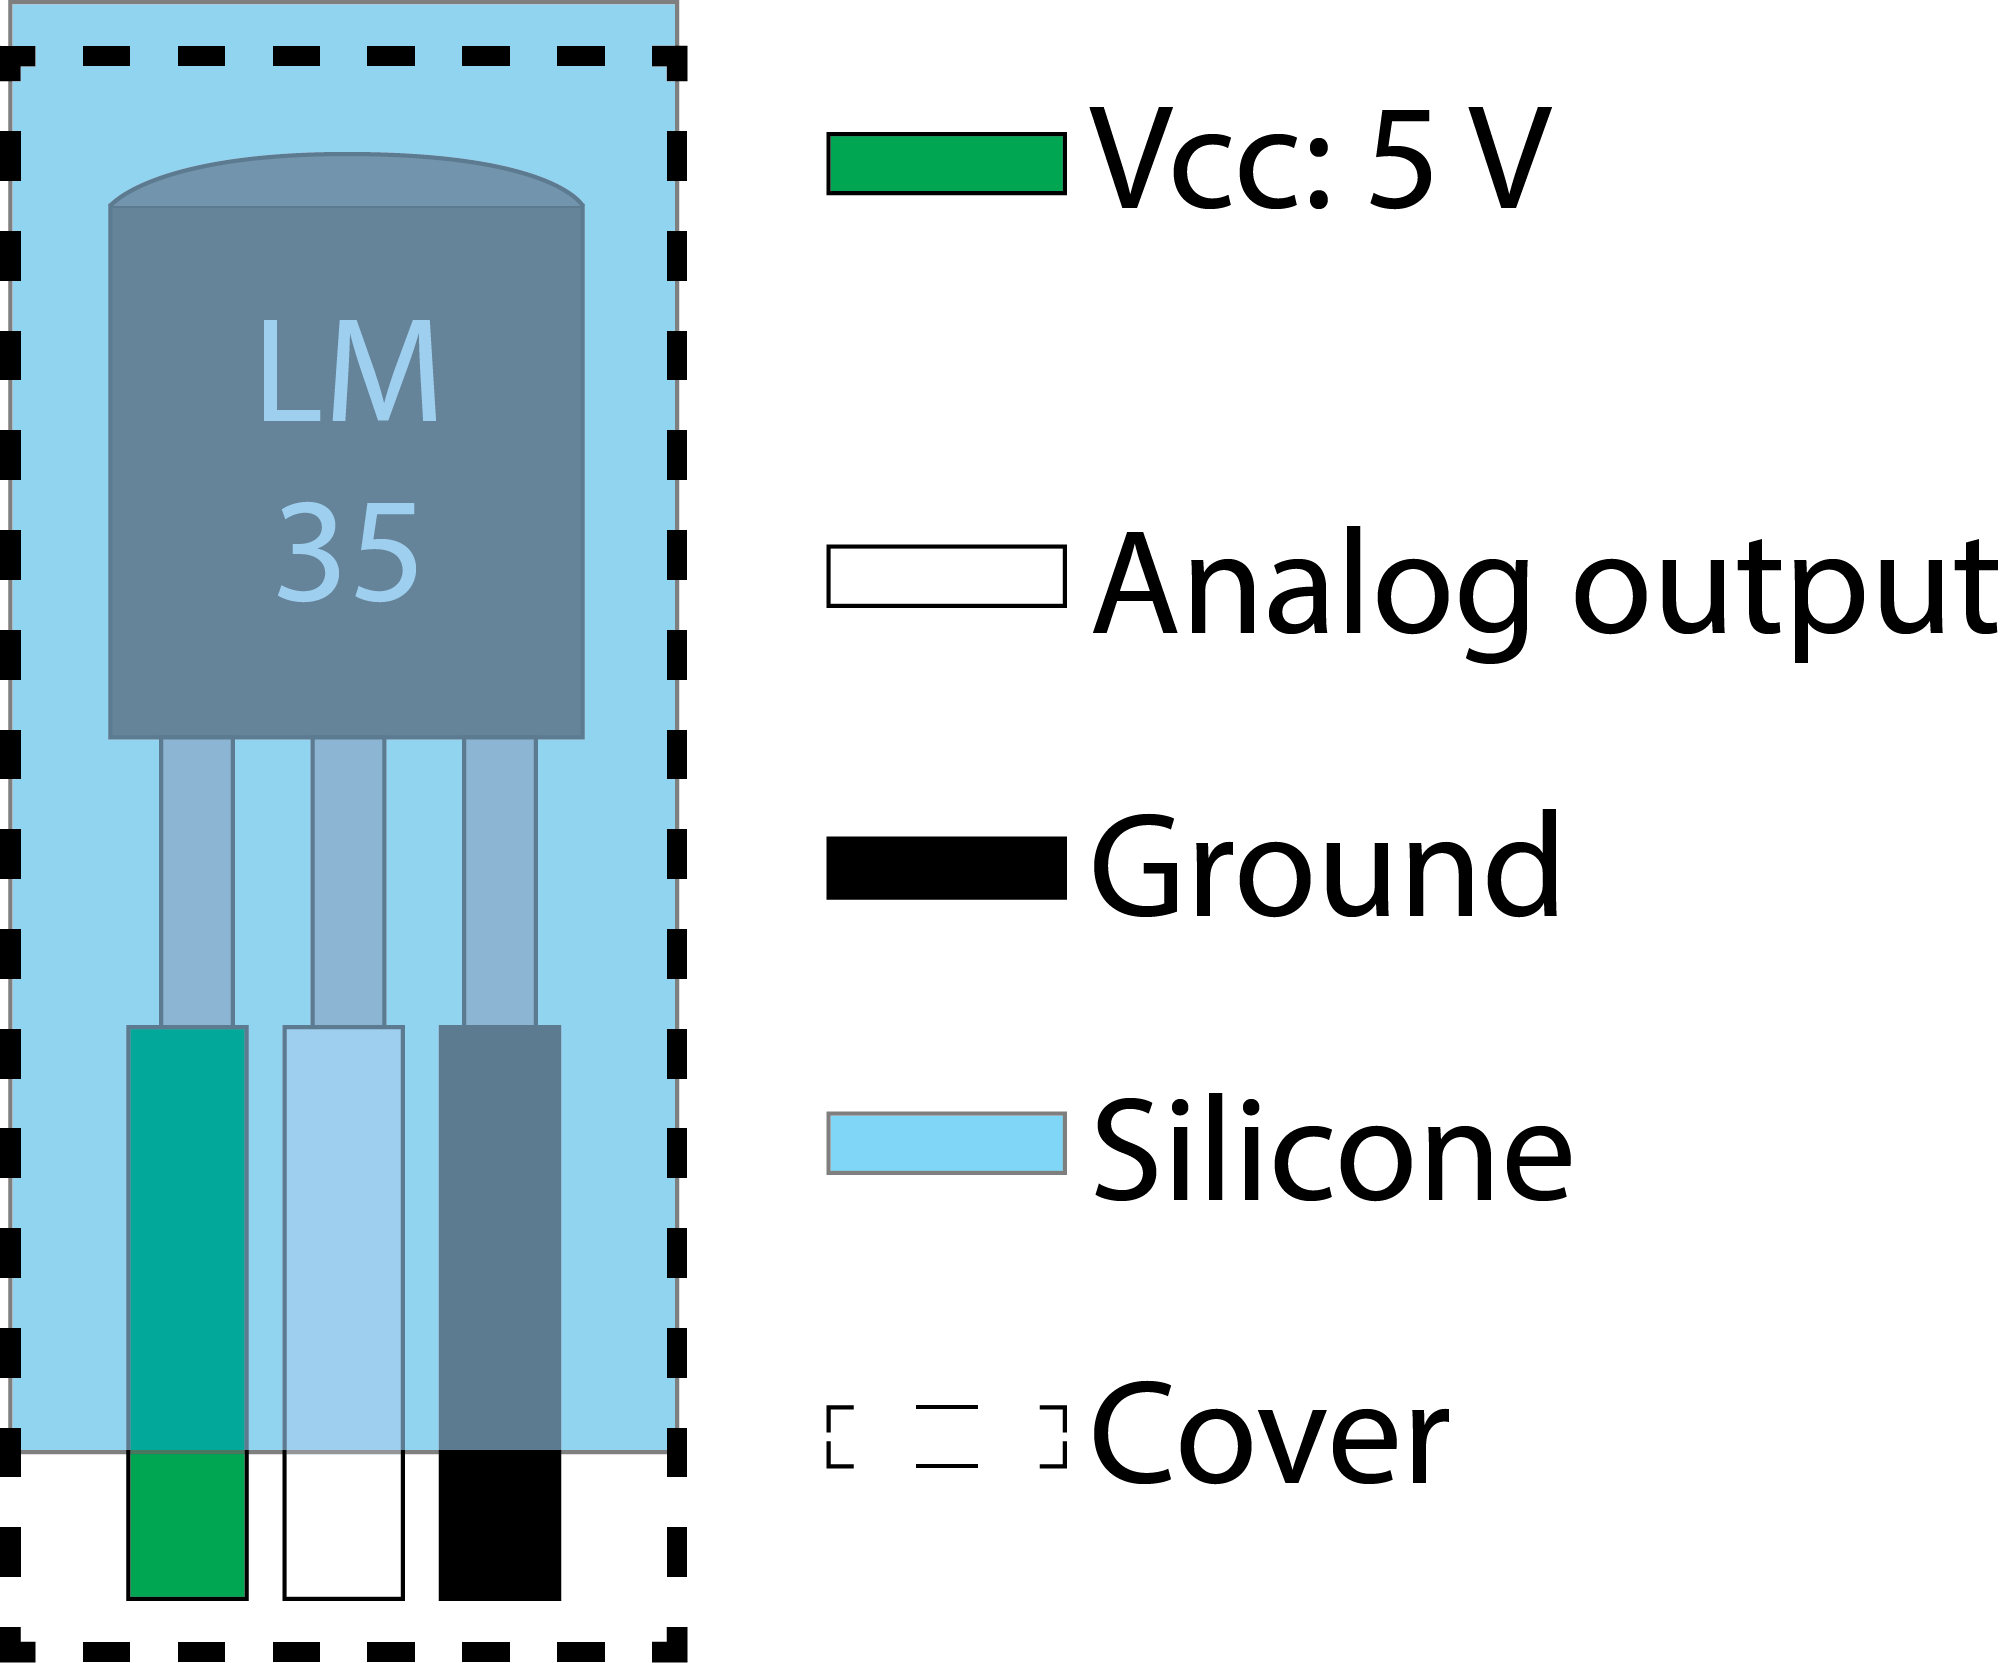
\includegraphics[width=\linewidth]{Figures/Sensor}
			\caption{Cableado del sensor LM35.}	
			\label{fig: sensors}
		\end{subfigure}
		\caption{Circuito del sistema de monitoreo de temperatura.}	
	\end{figure}

	Los sensores a su vez fueron conectados a un microcontrolador ATtiny 13 \cite{attiny13}.